\section{Android System Architecture}
\label{sec:bg_architecture}

The 5 layers that compose Android at the software level are shown in
Figure~\ref{fig:bg_architecture}\footnote{via:\url{http://en.wikipedia.org/wiki/Android\_(operating_system)\#Linux}}. Below
there is a brief overview of the Android system architecture \cite{ref13}:
\begin{enumerate*}
  \item The bottom layer is the \textit{Linux Kernel}, a slightly modified version of the standard one. The improvements are aimed at adapting the kernel to the hardware constraints of the mobile devices. 
  \item The libraries layer is a set of C/C++ essential C libraries rewritten to support ARM architecture. These libraries are accessible from the application framework. 
  \item The runtime is based on the dalvik virtual machine, with its specific libraries, and a collection of core libraries, specifically the interoperability libraries of the Java programming language. Since version 4.4 (codename Kitkat) it is written in C++. 
  \item The Application Framework, written in Java and interpreted by the DVM, is the main layer of the android framework and provides a rich set of components used by the applications to access the device functionalities. It contains also background processes that manages running applications and interoperability between them. 
  \item The last and higher layer is the Applications layer. Applications are built on top of the Applications Framework and provide the interfaces end users interact with. Most of the apps are written in Java but developers are also free to integrate it with native code for different purposes (e.g. games that extensively use GPU).
\end{enumerate*}

\begin{figure}[!h]
    \centering
    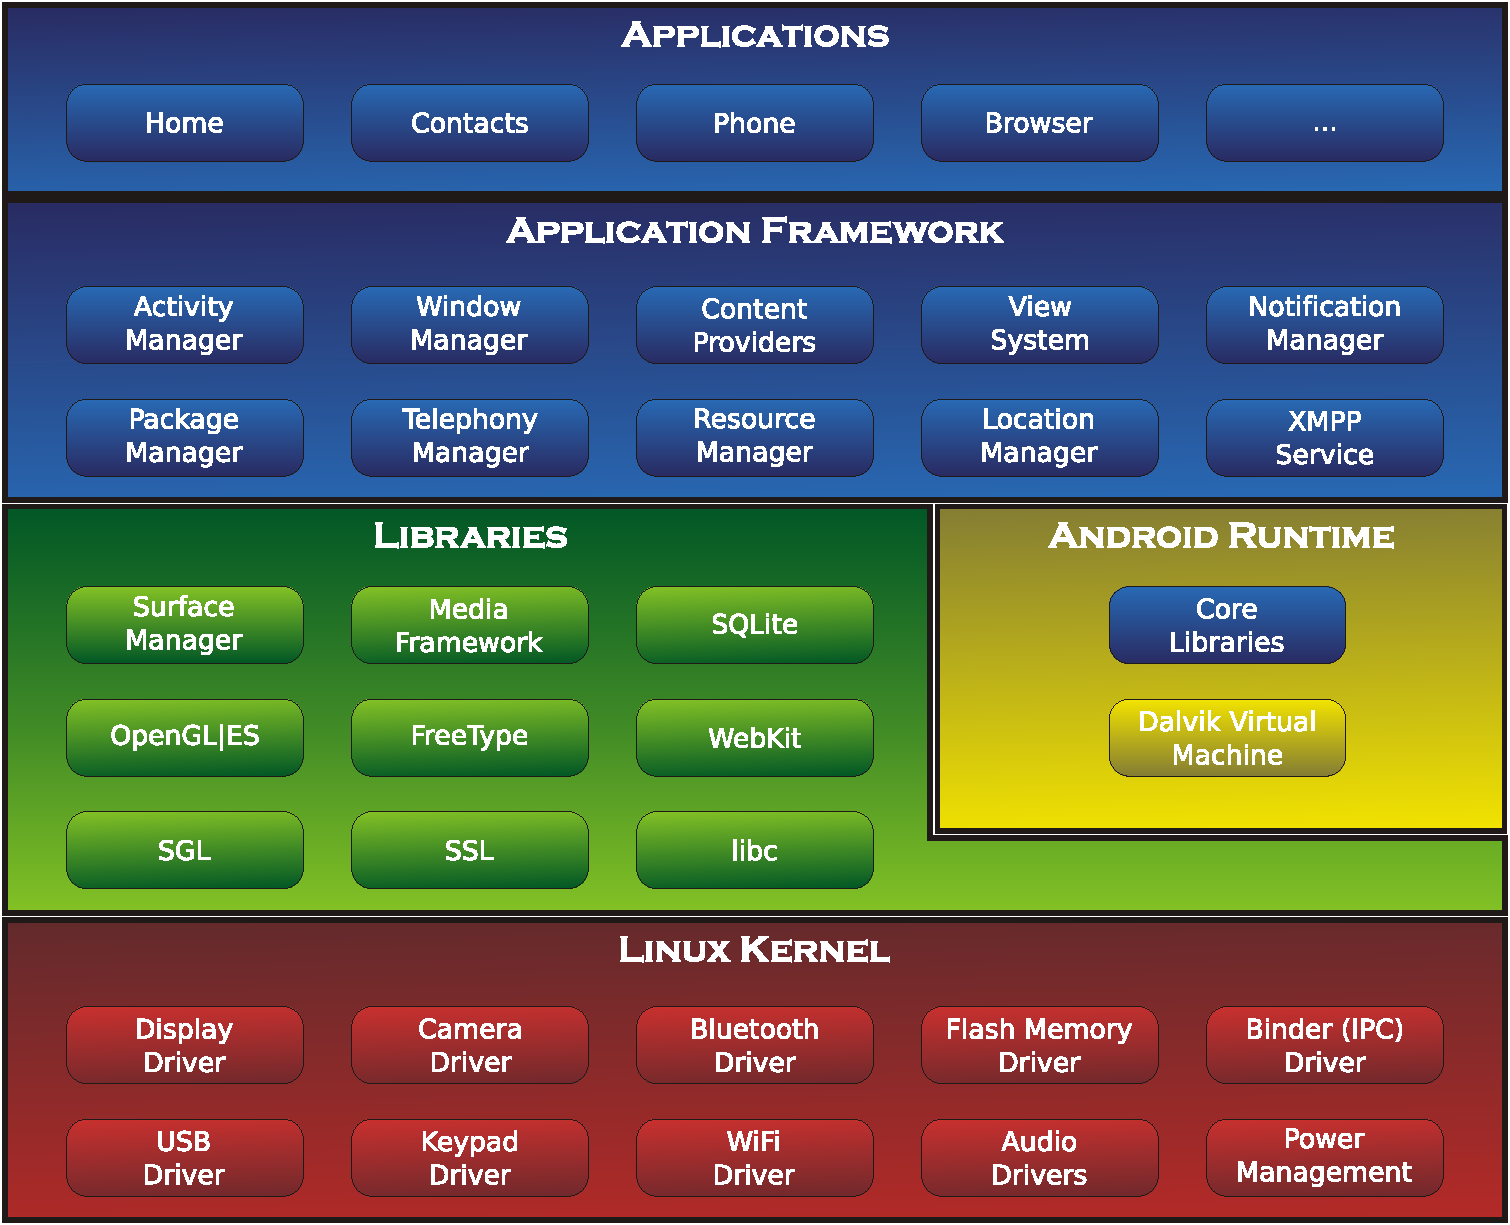
\includegraphics[width=1\textwidth]{./img/architecture/architecture.pdf}
    \caption{Android low level system architecture}
    \label{fig:bg_architecture}
\end{figure}
